\section{Calibration Campaigns}\label{sec:CalibCampaigns}
\subsection{Radioactive Sources}
For the calibration of the LSV detector response and the TPC's response to electron recoils (ER) we selected $^{57}$Co, $^{133}$Ba and $^{137}$Cs. In a later calibration campaign also $^{22}$Na has been deployed. They allow a cross-calibration with $^{83m}$Kr, that has been injected in the Ar recirculation system during dedicated campaigns and the internal $^{39}$Ar, as they cover the energy range of $^{39}$Ar (see also Table~\ref{tbl:GammaSources} and Fig.~\ref{fig:GammaSources_Ar39spectrum}). %As the interaction length increases with energy in LAr, the different gamma sources allow also to probe different regions of the TPC active volume.  
\mymarginpar{possible upgrade for fig.16: all measured spectra overlayed at a fixed HV: 83mKr, Co57, Ba133, Cs137 (either null field or 200 V/cm) - ask Brianne? Also for her thesis?}

After a preselection of gamma source energies, detailed studies with the DarkSide Monte Carlo G4DS \cite{DS50:G4DS:paper} were performed to select appropriate source activities and check the feasibility and physics reach of various deployment positions. Considering also constraints from the LSV and TPC DAQs, sources with suitable activities were identified for deployment (Table~\ref{tbl:GammaSources}).

Energy variables are calibrated in photo-electrons (PE) using dedicated Laser calibration runs, in which the single PE charge spectra for each PMT are fitted and a PE-charge gain is determined. 
These Laser runs are also an integral part of a calibration campaign requiring a Laser run at least on each change in DAQ or CALIS configuration, such as drift field changes or source position changes.

\begin{figure}[htbp]
 \centering
 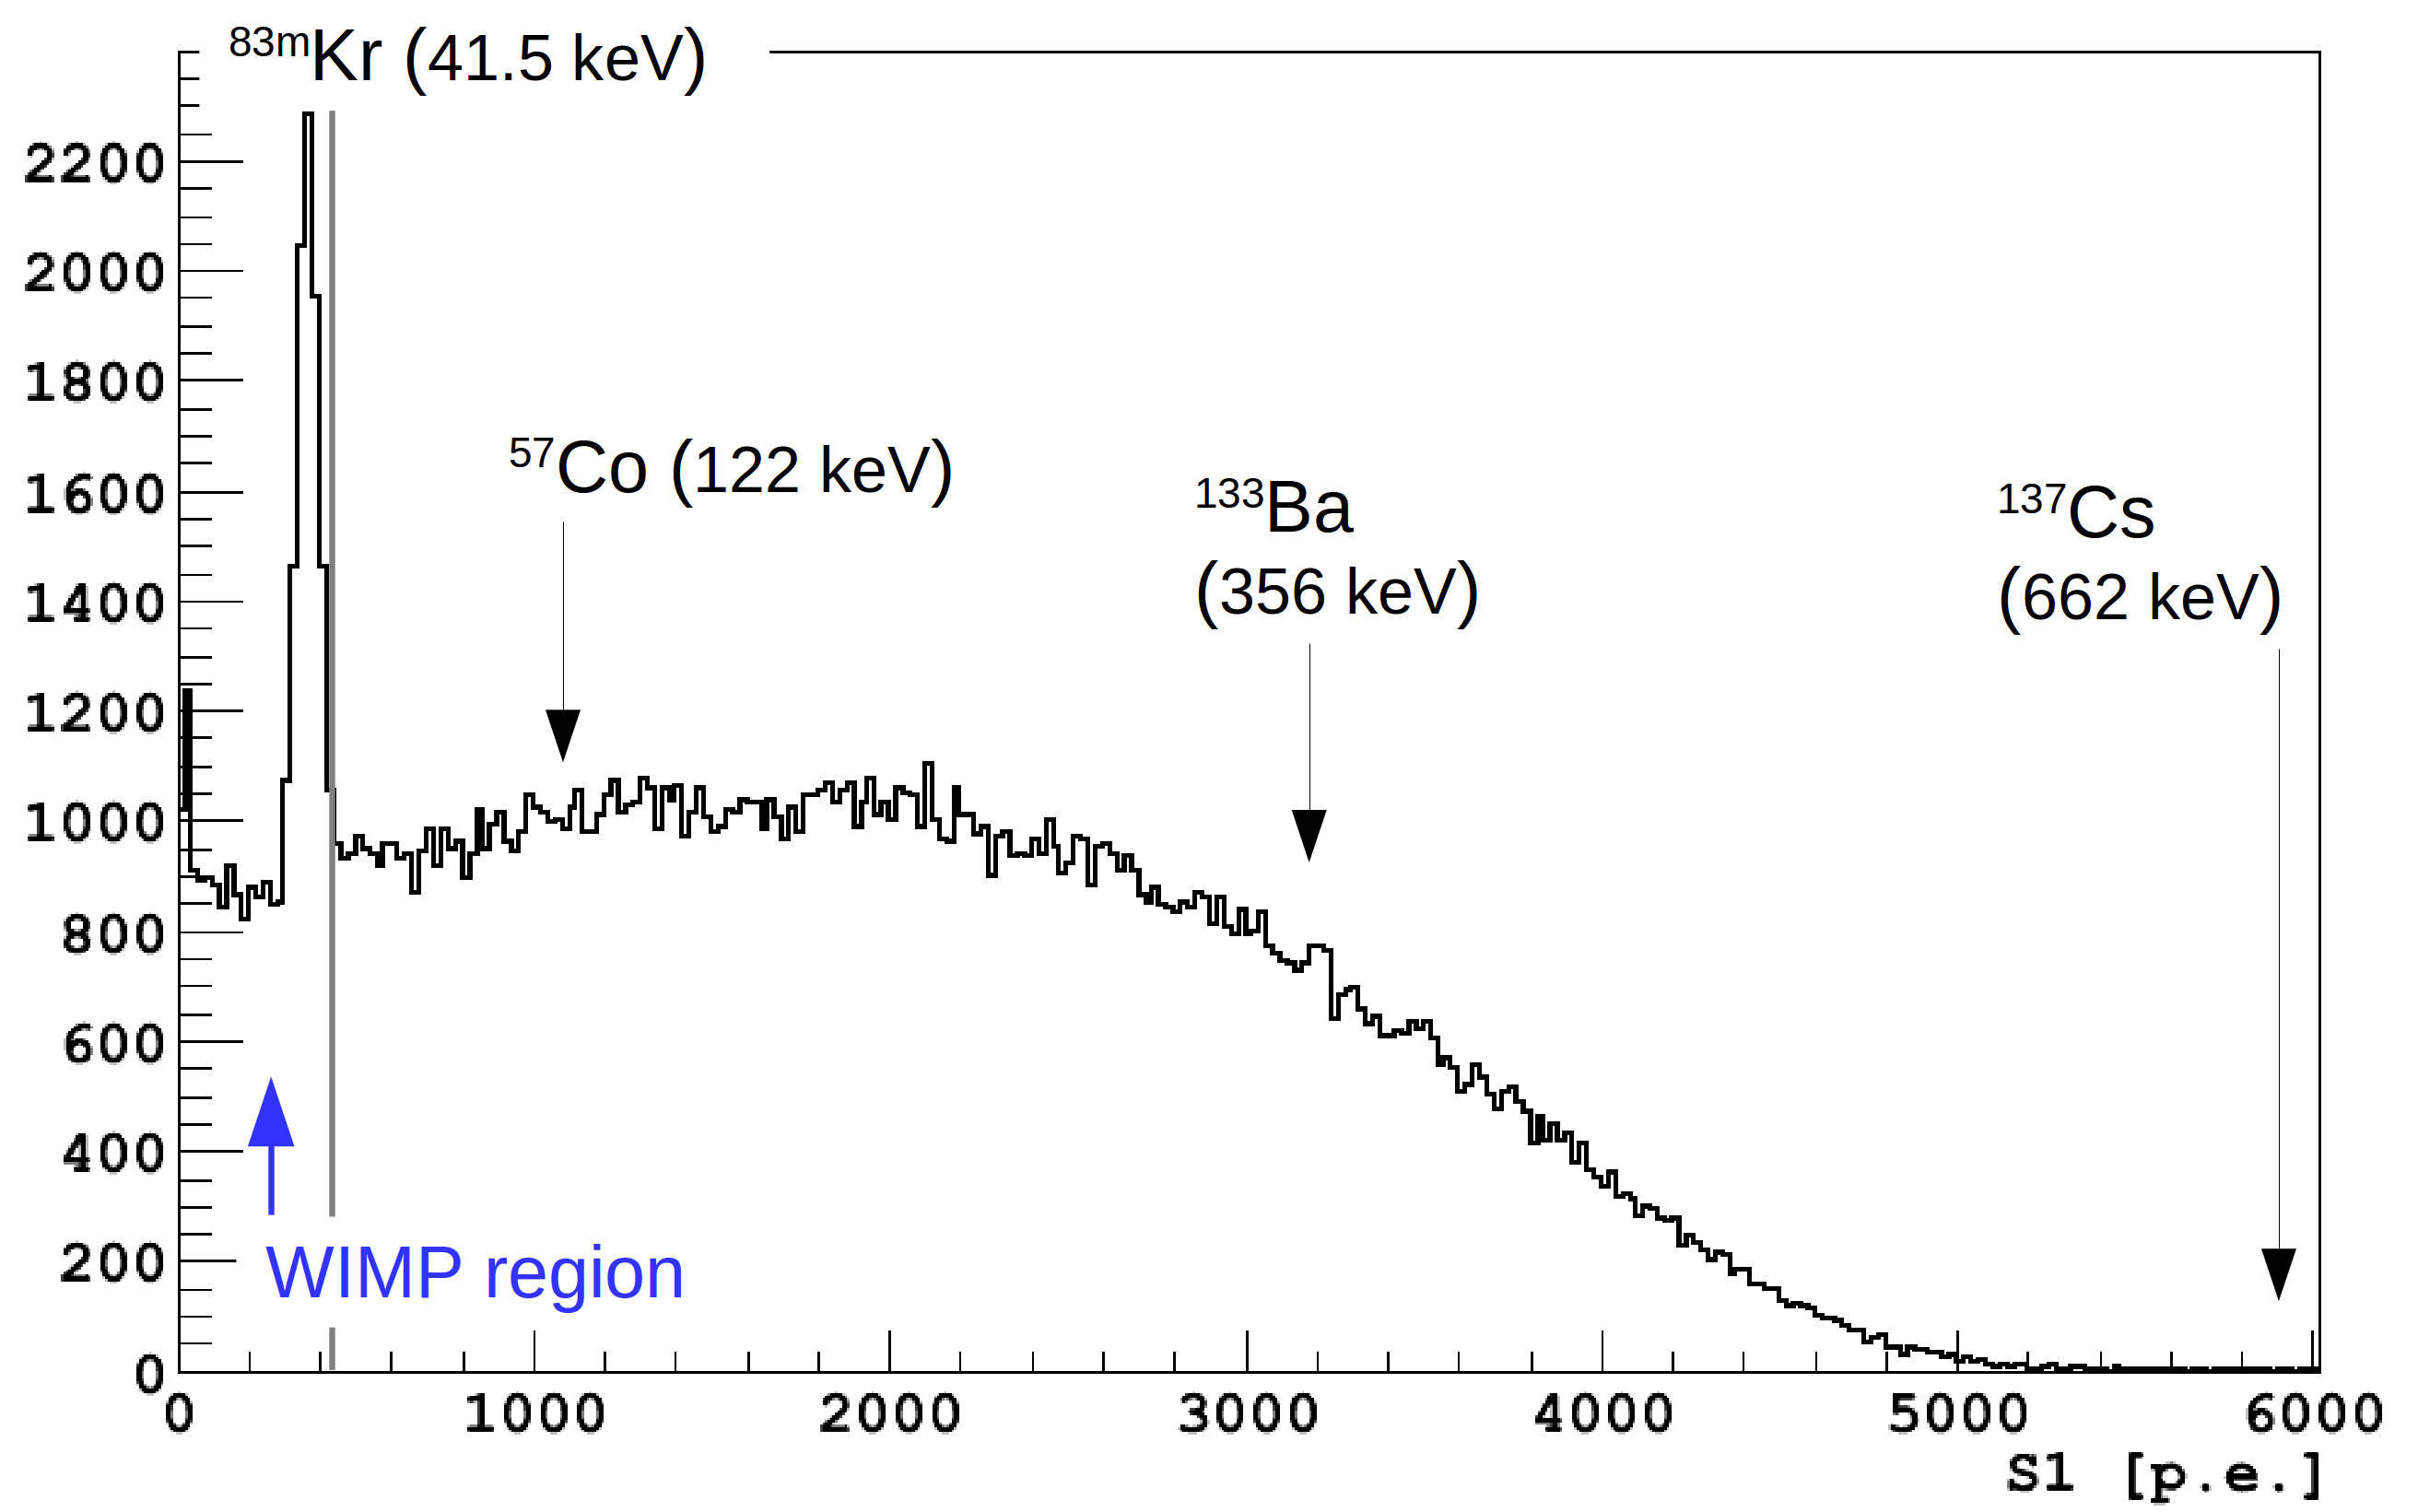
\includegraphics[width=0.8\textwidth]{Figures/GammaSources_Ar39spectrum.png}
 \caption{Scintillation spectrum (S1) at null field showing a $^{83m}$Kr peak on the $^{39}$Ar $\beta$ spectrum. The energies of the three gamma sources are indicated and cover the full range of the $^{39}$Ar spectrum.
\label{fig:GammaSources_Ar39spectrum}}
\end{figure}

\begin{table}[htbp]
\caption{Gamma sources deployed in DS-50, $^{39}$Ar and $83m$Kr \cite{lippincott-kr}. Interaction length is in LAr. Activity of $^{39}$Ar has been approx. 50 Hz during AAr filling and negligible in the UAr phase. The Kr source activity varied from campaign to campaign, but was in the range of a few Bq to some tens of Bq.} %\cite{Lippincott:83mKr}
\centering
\begin{tabular}{|l|l|l|l|l|l|}
\hline
\textbf{source} & \textbf{type} & \textbf{energy} & \textbf{half life} & \textbf{interact. length} & \textbf{activity} \\ \hline
$^{57}$Co & $\gamma$ & 122 keV & 0.744 y & 4.4 cm & 35 kBq \\ \hline
$^{133}$Ba & $\gamma$ & 356 keV & 10.54 y & 7.5 cm & 2 kBq \\ \hline
$^{137}$Cs & $\gamma$ & 662 keV & 30.2 y & 9.5 cm & 0.65 kBq \\ \hline
$^{22}$Na & $\gamma$ & $2\cdot 511$ keV + 1274 keV & xxx y & xxx cm & 11 kBq \\ \hline\hline
$^{39}$Ar & $\beta$ &  565 keV endpoint& xxx y & sub-mm & 50 Hz \\ \hline
$^{83m}$Kr & 2 $\beta$ &  32.1 keV + 9.1 keV & xxx y & sub-mm & \\ \hline

\end{tabular}
\label{tbl:GammaSources}
\end{table}
\mymarginpar{get the numbers for Na22 in the table}

\subsection{Timeline of the Calibration Campaigns and Stability}
Between October 2014 and April 2016 the following calibration campaigns have been performed:
\begin{itemize}
\item The first extensive campaign involving all gamma sources and both the high and low activity AmBe neutron source took place in October and November 2014 at LNGS\mymarginpar{has LNGS been introduced?}. The TPC was filled with atmospheric argon\mymarginpar{has atmospheric argon been introduced and underground argon?} with an inherent trigger rate of approx. 50 Hz from $^{39}$Ar. The liquid scintillator of the LSV contained a PC only scintillator with $<0.1 \%$ TMB and 1.4 g/l PPO as wavelength shifter.
%Fig.~\ref{???} shows the different configurations in which data has been taken as a function of source energy, source position and drift field.

\item In January and February 2015 a second campaign focusing on the LSV calibration using the low activity AmBe source was performed. Prior to that the LSV has been reconstituted with 5 \% TMB\mymarginpar{what does 5 \% TMB mean? weight \%, volume \%?}. Two deployments were performed at two different PPO concentrations (0.7 g/l and 1.4 g/l), allowing to study the impact of the PPO concentration on alpha and gamma quenching. (1.4 g/l is our nominal PPO concentration, see also Fig.~\ref{fig:LSV:Calib}, right)

\item In August 2015 a $^{22}$Na source has been deployed next to the cryostat for TPC calibration. This was the first gamma source calibration campaign after the UAr deployment within \dsf.
\item In December 2015 an $^{241}$Am$^{13}$C neutron source has been deployed, allowing an in-depth study of the detection efficiency of the prompt neutron recoil signal in the absence of the correlated 4.4 MeV gamma, obfuscating the neutron recoil signal in case of an AmBe source.
\end{itemize}

As shown in Fig.~\ref{fig:LSV:Stability}\mymarginpar{instead of the timeline by Yann (DocDB 1232) I would like to show the Co60 and a rate stability plot - in progress.} the calibration campaigns have not affected negatively the light yield or introduced radioactivity into the LSV.

\begin{figure}[htbp]
\centering
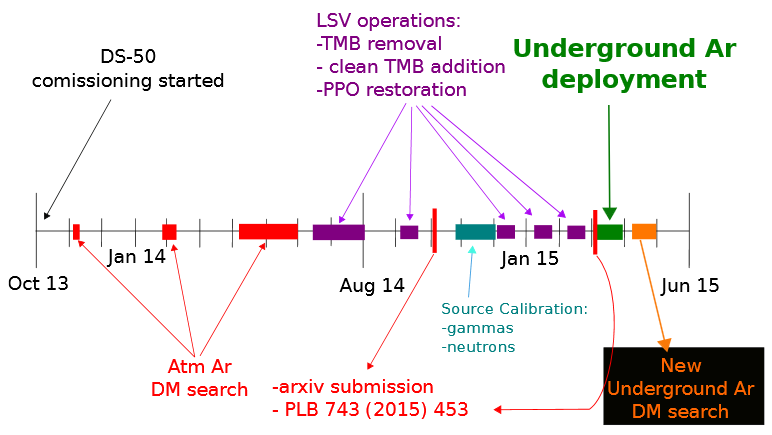
\includegraphics[width=0.7\textwidth]{./Figures/Yann_timeline.png}
\caption{In black the stability of the LSV LY is monitored using internal $^{60}$Co emitted from the cryostat steel, in blue the stability of the rate of radioactivity in the LSV is shown. Before and after calibration campaigns both the LY and the rate remain unaffected.
\label{fig:LSV:Stability}}
 \end{figure}


\subsection{TPC Calibration}
A few calibration results are shown have been collected from DarkSide papers to illustrate the quality of the acquired calibration data.

\subsubsection{$^{57}$Co S1 energy}
Fig.~\ref{fig:CalibData:Co57} shows a data-MC comparison of the scintillation signal S1 spectrum of a $^{57}$Co calibration source deployed next to the cryostat and close to the TPC active volume center. Overlayed is the S1 distribution from an equivalent selection of G4DS MC simulation \cite{DS50:G4DS:paper}.\mymarginpar{The plot is from Paolo's G4DS talk \@ DS2016, UCLA. Ideally one could get an official copy from the MC paper.}

\begin{figure}[htbp]
\centering
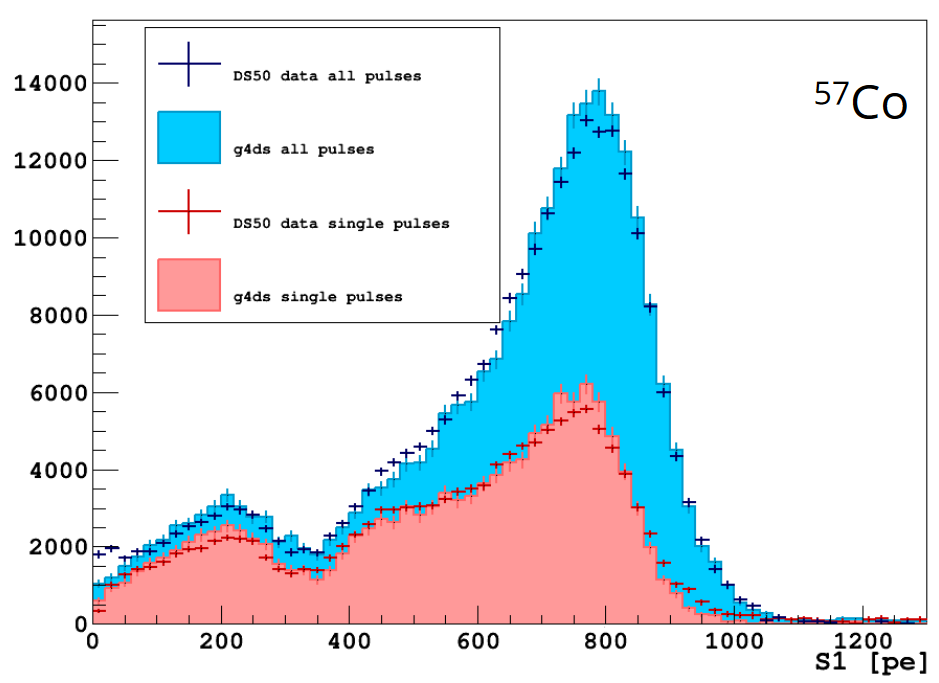
\includegraphics[width=0.7\textwidth]{./Figures/57Co_Paolo_G4DS_UCLA.png}
\caption{Data-MC comparison for the $^{57}$Co source deployed next to the cryostat. In the magenta distribution a single-site interaction requirement has been imposed as for dark matter events and for the blue distribution this constraint has been removed \cite{DS50:G4DS:paper}.
\label{fig:CalibData:Co57}}
 \end{figure}


\subsubsection{F90 distribution from $^{241}$Am$^9$Be neutron data}\label{sec:CalibData:NR}

Fig.~\ref{fig:CalibData:F90} shows good agreement between F90 medians and S1 spectra measured from $^{241}$Am$^9$Be neutron data and those derived from \SCENE\ measurements, which have been used to determine the nuclear recoil energy scale and NR acceptance regions for the WIMP dark matter search \cite{ds:ds-50-PLB, DS:2ndPaper}.
\begin{figure}[htbp]
\centering
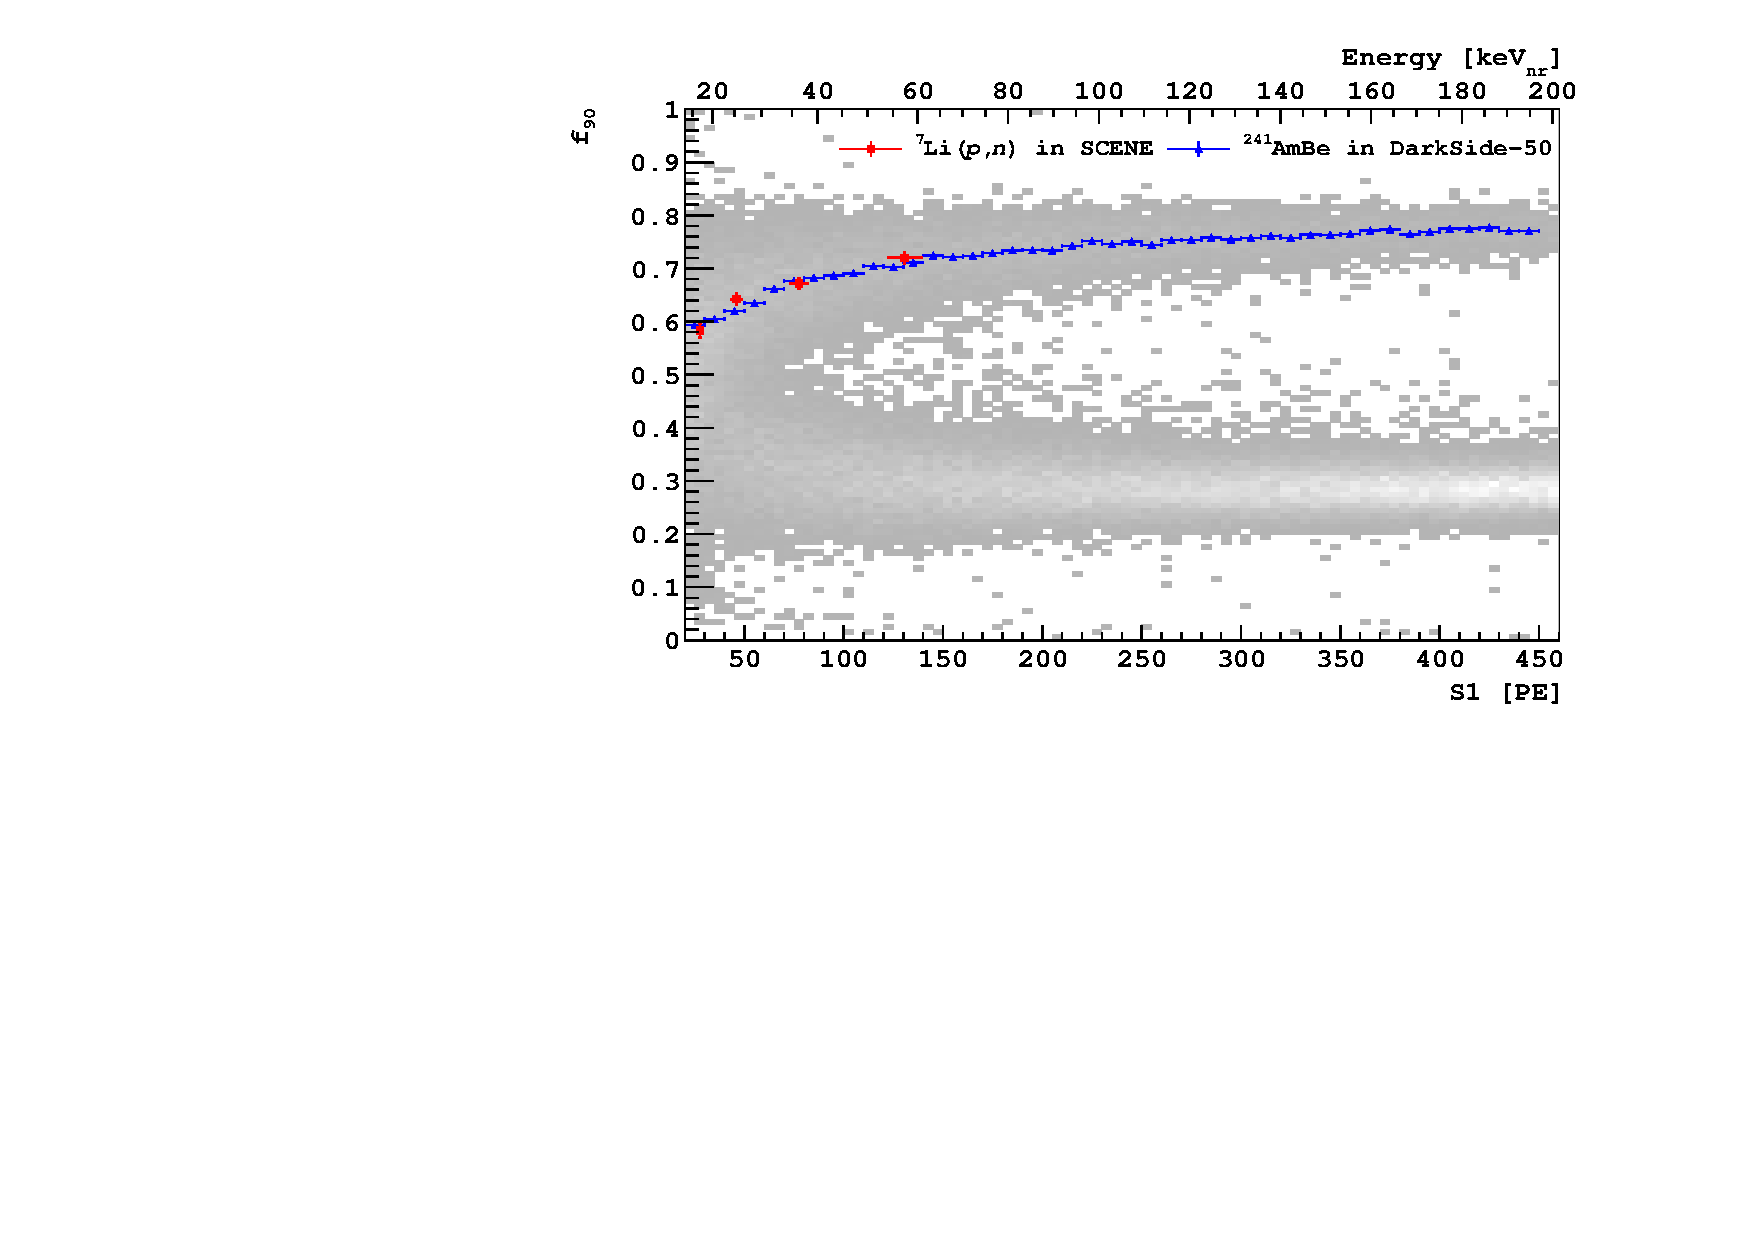
\includegraphics[width=0.7\textwidth]{./Figures/DSf-UArAmBeDMSStCut.pdf}
\caption{Plot of F90 vs. scintillation signal S1 from a high rate AmBe neutron source calibration of \dsf\ in grey, the upper NR band from the AmBe calibration and lower ER band from $\beta$-$\gamma$ backgrounds are visible. Overlayed are \FNinety\ \NR\ median vs. \SOne\ from a high-rate {\it in situ} AmBe\ calibration (blue) and scaled from \SCENE\ measurements (red points) \cite{scene2}. There is very good agreement between the two.  The high source intensity and correlated neutrons and $\gamma$-ray emission by the AmBe source contribute events outside the nuclear recoil and electron recoil bands. (reproduced from \cite{DS:2ndPaper})\label{fig:CalibData:F90}\label{fig:DSf-UArAmBeDMS}} 
\end{figure}


\subsubsection{Source position}
Tests at LNGS established the deployment system's positioning accuracy to be about $\pm$1 cm after a 7 meter journey into the DarkSide-50 detector.
%comment to the "about $\pm ": the tilde $~ \pm$ did not show up at all in the output.
During the first calibration campaign several runs have been taken with the source at its central position (731000 motor step counts). Fitting the t$_{drift}$ distribution at that position a systematic shift vs.~time has been observed (Fig.~\ref{fig:SourcePosition}, right). Overall on average the source position has been positioned 157.4 mm below the grid with an RMS of 10.1 mm. Following that observed shift the deployment procedures have been revised to avoid such a time dependency in the future and to improve the deployment precision. It is worth mentioning though that this does not induce significant uncertainties for dark matter searches, as the t$_{drift}$ distribution can be measured in-situ on a per-run basis.
\begin{figure}[htbp]
\centering
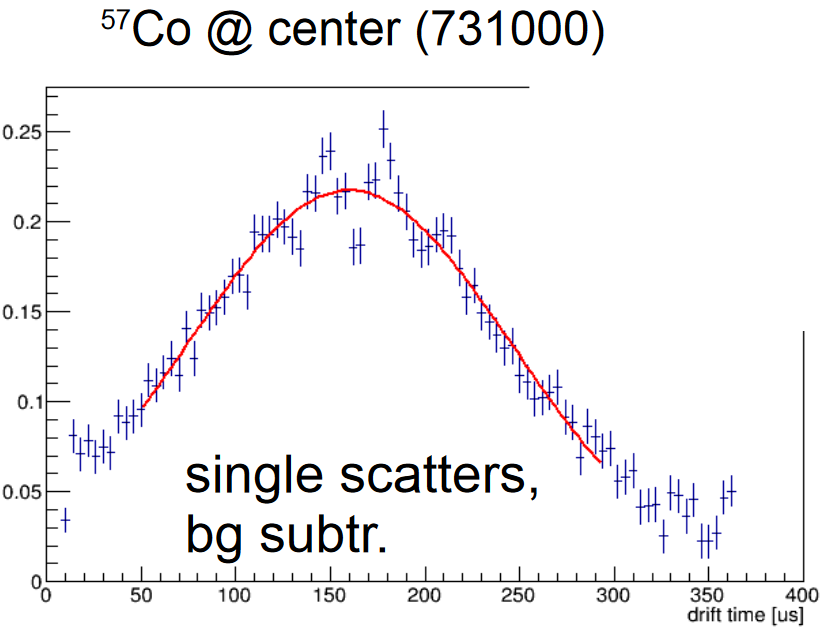
\includegraphics[width=0.48\textwidth]{./Figures/Tdrift_distribution_Co57_DocDB1288.png}
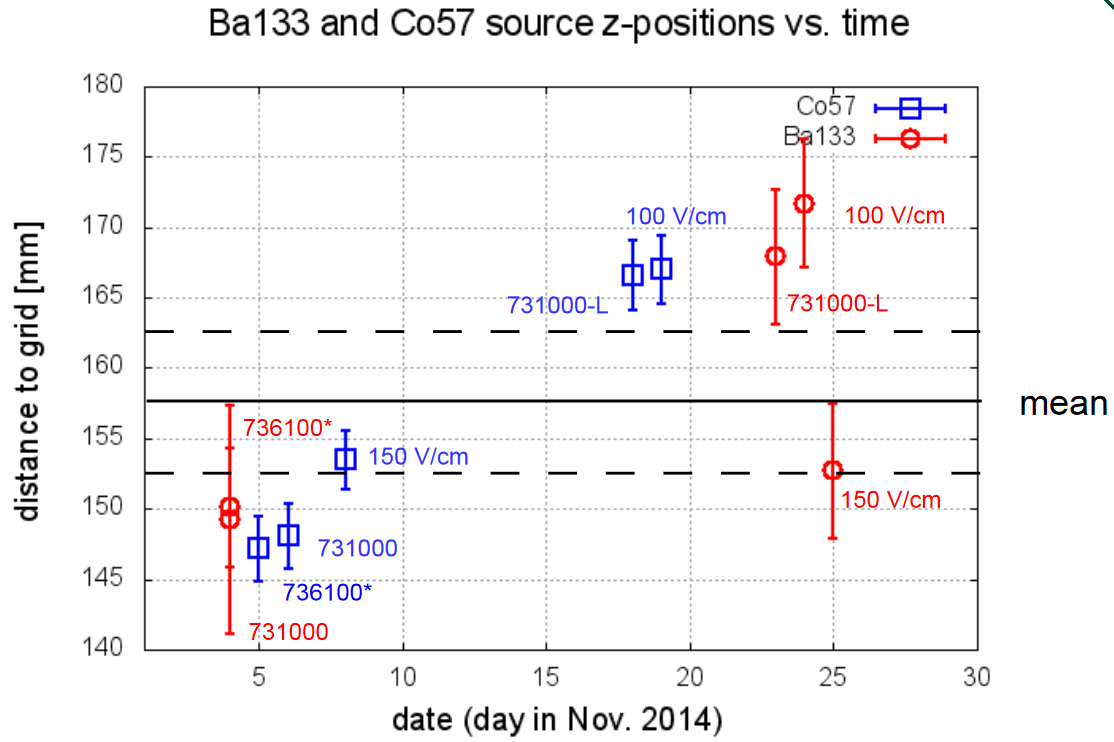
\includegraphics[width=0.48\textwidth]{./Figures/SourcePosition_vs_time_DocDB1288.png}
\caption{\textit{left:} A t$_{drift}$ distribution encoding the z-position of the $^{57}$Co deployed next to the TPC center.
\textit{right:} Shift of source position relative to the TPC grid as a function of time when deployed to the same place.
\label{fig:SourcePosition}} 
\end{figure}

For the XY position the distribution of the azimuthal angle in the XY plane has been studied and a mean of 139 degrees has been observed with an RMS of 1.2 deg. (One degree corresponds to 6 mm at the outer cryostat, where the source is positioned.) However an independent XY reconstrution algorithm gave 142.5 degrees with an RMS of 0.8 deg, so that systematic uncertainties dominate over the XY precision \cite{DS:XY:paper}.\mymarginpar{This is from DocDB 1288. Ideally one could cite a XY paper here, which is not published yet.}


%%%%%%%%%%%%%%%%%%%%%%%%%%%%%%%%

\subsection{Liquid Scintillator Veto}\label{sec:LSV:gammasources}

In Fig.~\ref{fig:LSV:Calib}, left a data-MC comparison of the LSV charge spectra from the $^{137}$Cs source deployed in the LSV next to the cryostat is shown \cite{DS50:G4DS:paper}.
In January and February 2015 the reconstitution of the LSV scintillator was completed and a second AmBe neutron source calibration of the LSV calibration was undertaken to further study the various neutron detection channels in the LSV. With a borated scintillator, a critical aspect of the neutron detection efficiency is the capability to observe the \brbortenground\
capture branch leading to a \enbortengroundalpha\ $\alpha$ + $^7$Li(g.s.) without the accompanying 478 keV $\gamma$-ray. As shown in Fig.~\ref{fig:LSV:Calib}, right the de-excitation channel is clearly observed at around 30 PE.

\begin{figure}[htbp]
\centering
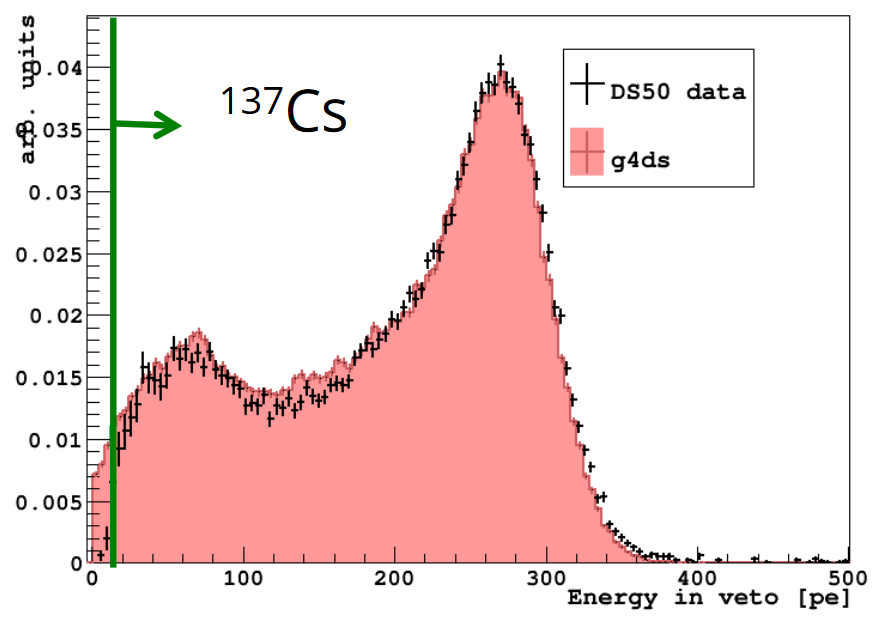
\includegraphics[width=0.48\textwidth]{./Figures/137Cs_Veto_Paolo_G4DS_UCLA.png}
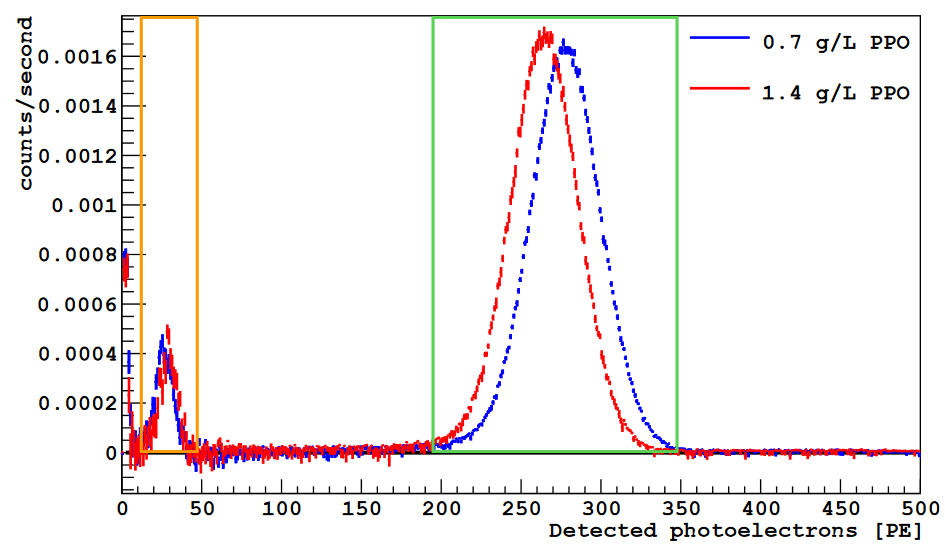
\includegraphics[width=0.48\textwidth]{./Figures/AmBe_LSV_VetoPaper.png}
\caption{\textit{left:} Data-MC comparison of the LSV charge spectra from the $^{137}$Cs source deployed in the LSV next to the cryostat \cite{DS50:G4DS:paper}.
\textit{right:} Clear detection of the neutron capture signal on $^{10}$B in the LSV leading to a \enbortengroundalpha\ $\alpha$ + $^7$Li(g.s.) at $\approx$ 30 PE (orange box). The
peak on the right at $\approx$ 270 PE (green box) is from the 93.6 \% of captures that lead to the $^7$Li excited state reaction, with the accompanying 478 keV-ray. The entries below 10 PE are due to PMT after-pulses. Data has been taken before and after varying the concentration of the wavelength shifter PPO in the scintillator with the source rotated 70 cm away from the cryostat. In both cases the deexcitation to ground state is clearly observed.\cite{DS50:VetoPaper}
\label{fig:LSV:Calib}} 
\end{figure}
